\documentclass[12pt,a4paper]{article}

% Paquetes necesarios
\usepackage[utf8]{inputenc}  % Codificación UTF-8
\usepackage[spanish]{babel}  % Español
\usepackage{amsmath, amssymb, amsthm}  % Paquetes matemáticos
\usepackage{graphicx}  % Para incluir imágenes
\usepackage[margin=1in]{geometry}  % Márgenes
\usepackage{lipsum}  % Texto de ejemplo
\usepackage{float}  % Para usar [H] en figuras
\usepackage{subcaption} % Para usar subfiguras
\usepackage{algorithm2e}  % Para escribir algoritmos
% \usepackage{algpseudocode}

% Configuración del título
\title{\textbf{Título del Artículo Matemático}}
\author{\textbf{Autor del Artículo}\\ Universidad o Institución}

\date{\today}

\begin{document}

% Portada
\begin{titlepage}
    \centering
    \vspace*{5cm}
    
    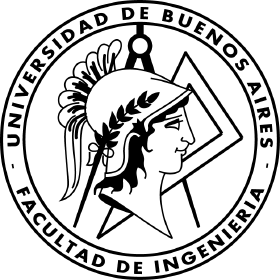
\includegraphics[width=0.4\textwidth]{logo-fiuba.png}\\[1cm]
    
    {\Huge \textbf{Trabajo Práctico 2}}\\[0.2cm]

    {\large \textbf{Aprendizaje Profundo}\\ Alejo Ordoñez}
    
    \vfill
    
    % {\large \today}
    {\large 27 de noviembre de 2024}
\end{titlepage}

\newpage
\tableofcontents

% Contenido principal
\newpage
\section*{Resumen}
En este trabajo se abordan el diseño, implementación y análisis de varias arquitecturas de redes neuronales. En particular, se cubren un perceptrón simple, un perceptrón multicapa, una máquina restringuida de Boltzmann, una red convolucional y un autoencoder. Se cubre el algoritmo de aprendizaje gradient descent, usando backpropagation para el cálculo de los gradientes, y se usa el algoritmo de preentrenamiento introducido en el trabajo de Hinton y Salakhutdinov (2006) para la de la máquina de Boltzmann.

\newpage
\section{Perceptrón simple}
El perceptrón simple es la unidad básica de una red neuronal. Es una neurona artificial que usa una función de activación escalón. La función mapea la entrada $\mathbf{x}$ (un vector de números reales) a una salida binaria $f(\mathbf{x})$:
$$
f(\mathbf{x}) = h (\mathbf{w} \cdot \mathbf{x} + b),
$$
donde $h$ es la función escalón, $\mathbf{w}$ es el vector de pesos, $\mathbf{x}$ es el vector de entradas y $b$ es el sesgo. El sesgo genera una traslación del límite de decisión, que es el hiperplano definido por $\mathbf{w} \cdot \mathbf{x} + b = 0$.
\begin{figure}[H]
    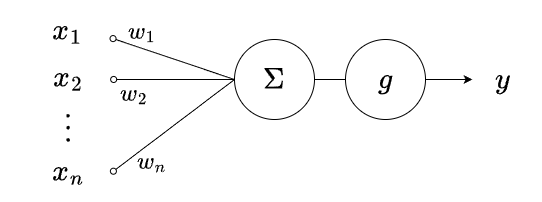
\includegraphics[width=0.7\textwidth]{img/simple_perceptron.png}
    \centering
\end{figure}
El entrenamiento de un perceptrón simple, consiste en la actualizar los pesos y el sesgo de acuerdo a
$$
w_i = \alpha (y - \hat{y}) x_i\\
b = \alpha -(y - \hat{y}),
$$
donde $\alpha$ es la taza de aprendizaje, el par $x, y$ es un ejemplo de entrenamiento y $\hat{y}$ es la salida del perceptrón.
En primer lugar se implementó un perceptrón simple que aprendió la función lógica AND de dos entradas.\\
La evolución del error durante el entrenamiento y la recta discriminadora aprendida por el perceptrón, $x_2 = -(w_1 x_1 = b) / w_2$, se muestran a continuación:
\begin{figure}[H]
  \subcaptionbox*{Evolución del error}[.45\linewidth]{
    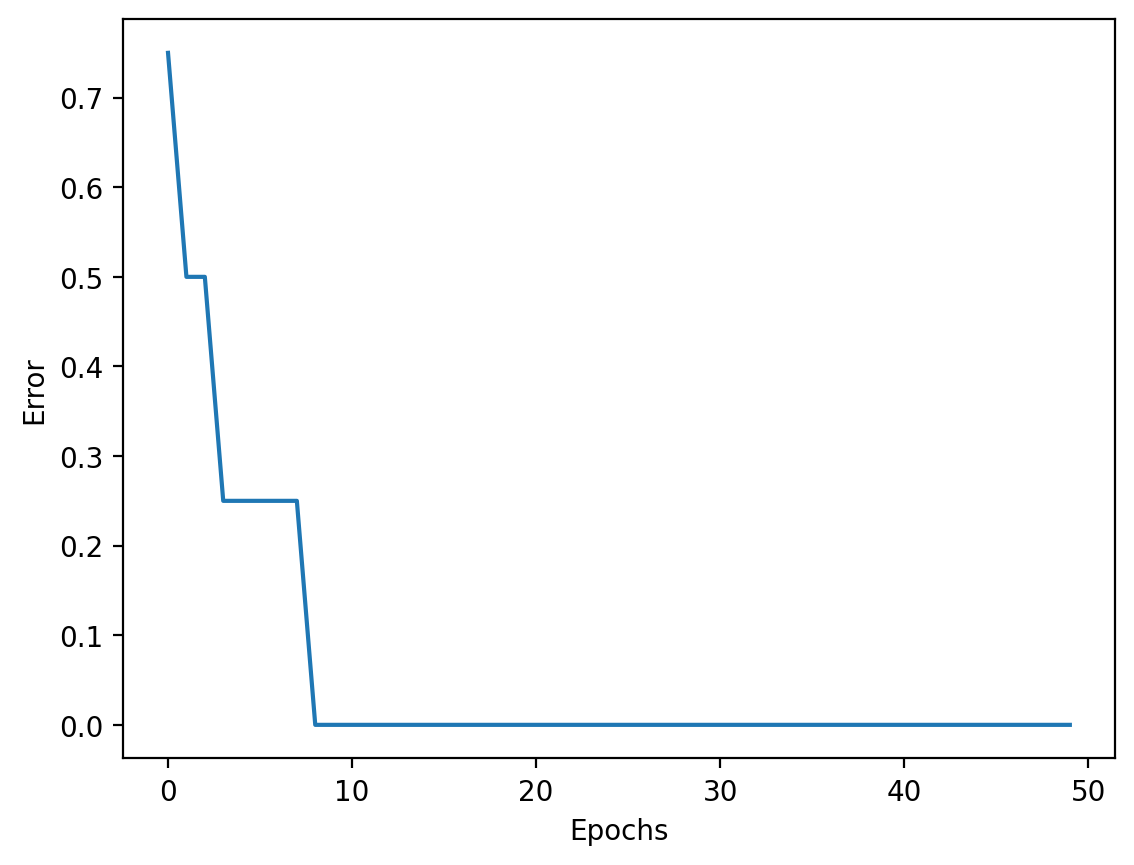
\includegraphics[width=\linewidth]{img/1-training_error.png}
  }
%   \hfill
  \subcaptionbox*{Recta discriminadora}[.45\linewidth]{
    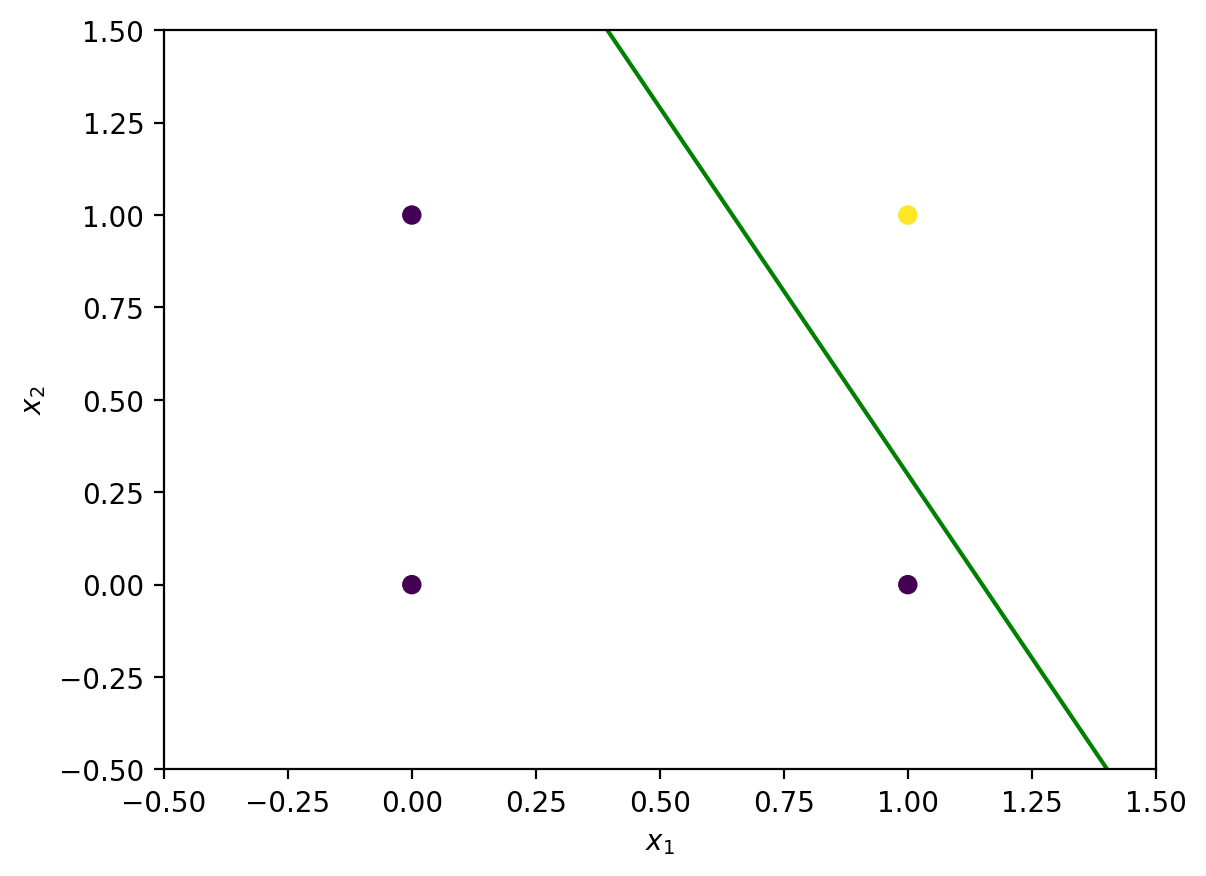
\includegraphics[width=\linewidth]{img/2-desicion_boundary.png}
  }
  \centering
\end{figure}
Seguidamente, se entrenaron perceptrones para que aprendiieran las funciones lógicas OR de dos entradas, y AND y OR de cuatro entradas. Los resultados se muestran a continuación:
\begin{figure}[H]
  \subcaptionbox*{Evolución del error}[.45\linewidth]{
    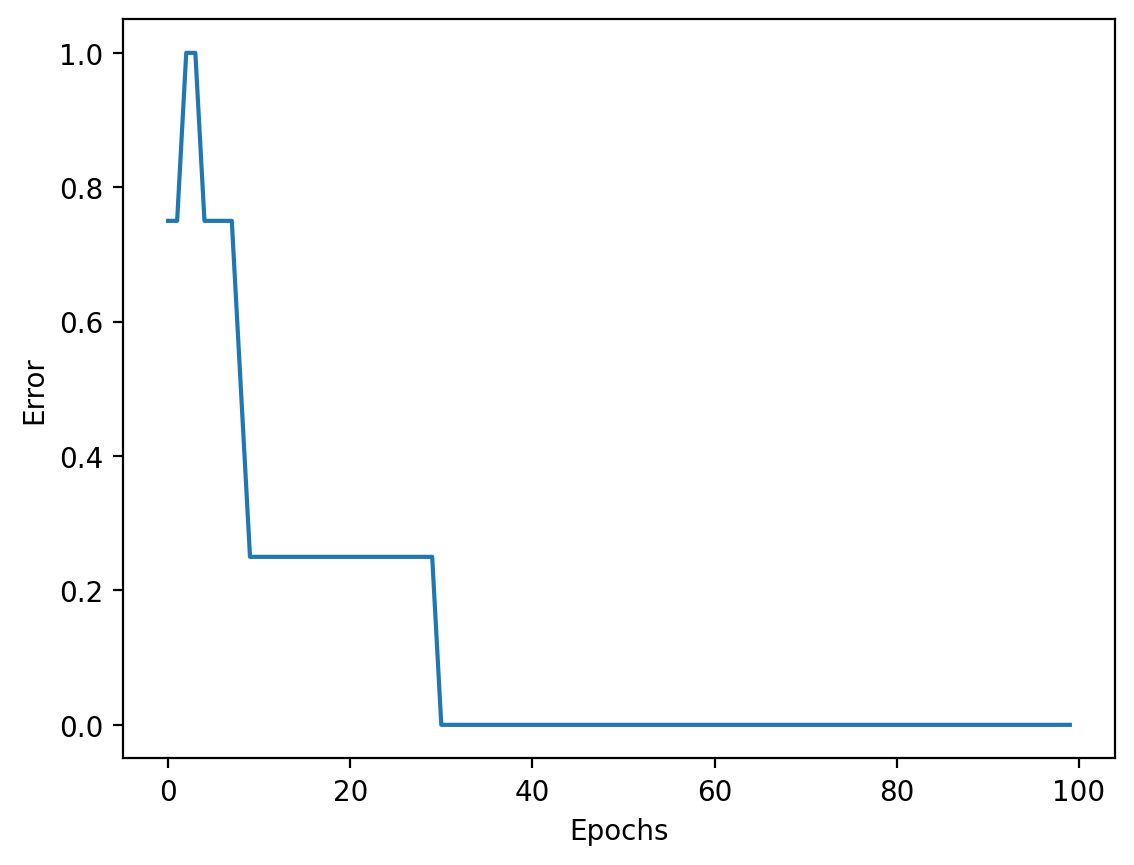
\includegraphics[width=\linewidth]{img/3-training_error.png}
  }
%   \hfill
  \subcaptionbox*{Recta discriminadora}[.45\linewidth]{
    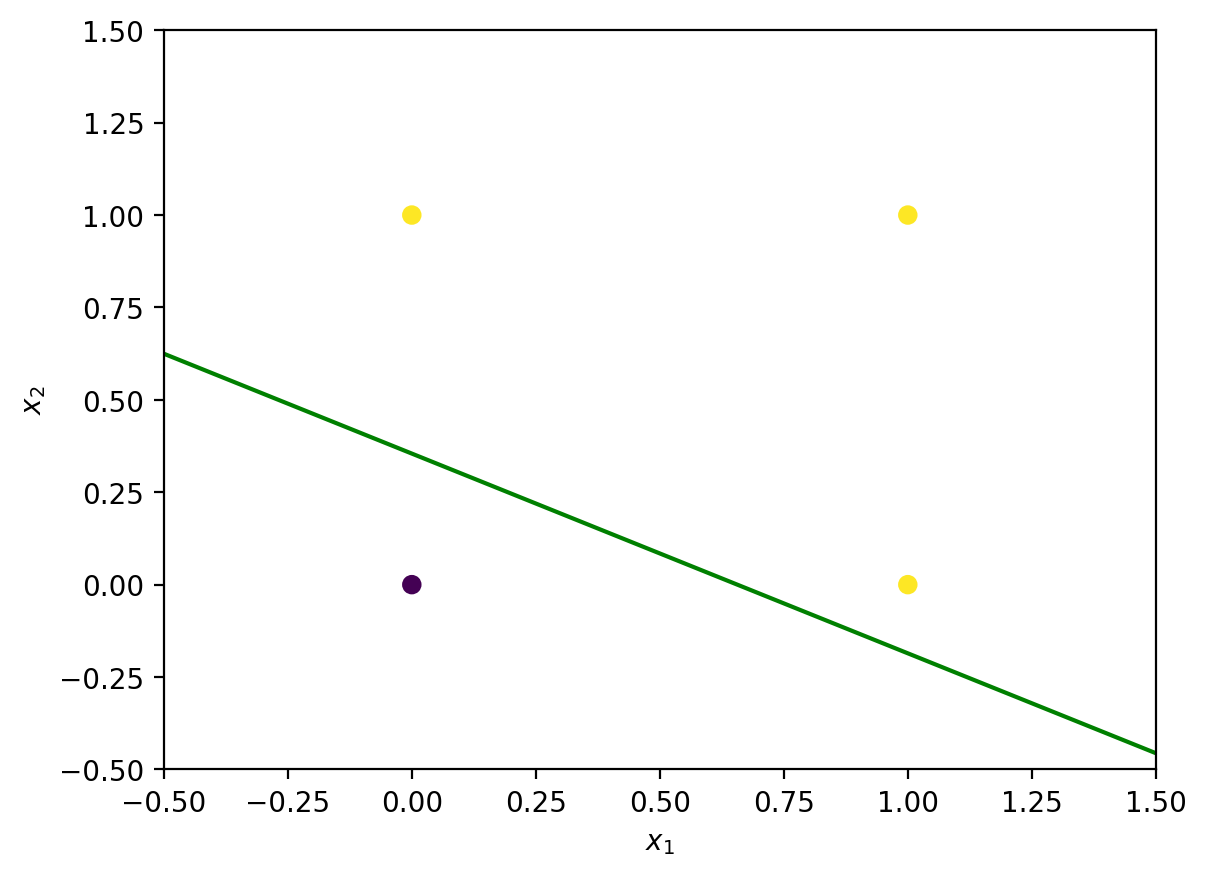
\includegraphics[width=\linewidth]{img/4-desicion_boundary.png}
  }
  \caption*{OR de dos entradas}
  \centering
\end{figure}
\begin{figure}[H]
  \subcaptionbox*{AND de cuatro entradas}[.45\linewidth]{
    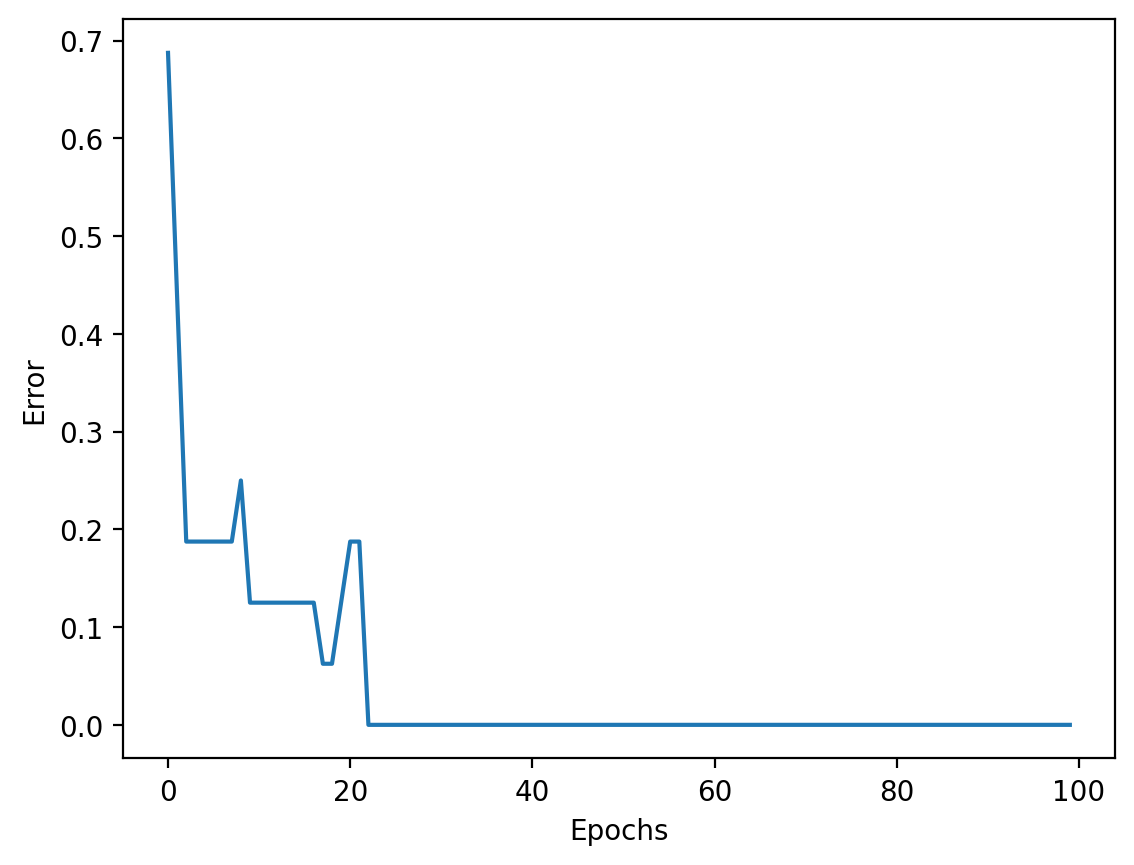
\includegraphics[width=\linewidth]{img/5-training_error.png}
  }
%   \hfill
  \subcaptionbox*{OR de cuatro entradas}[.45\linewidth]{
    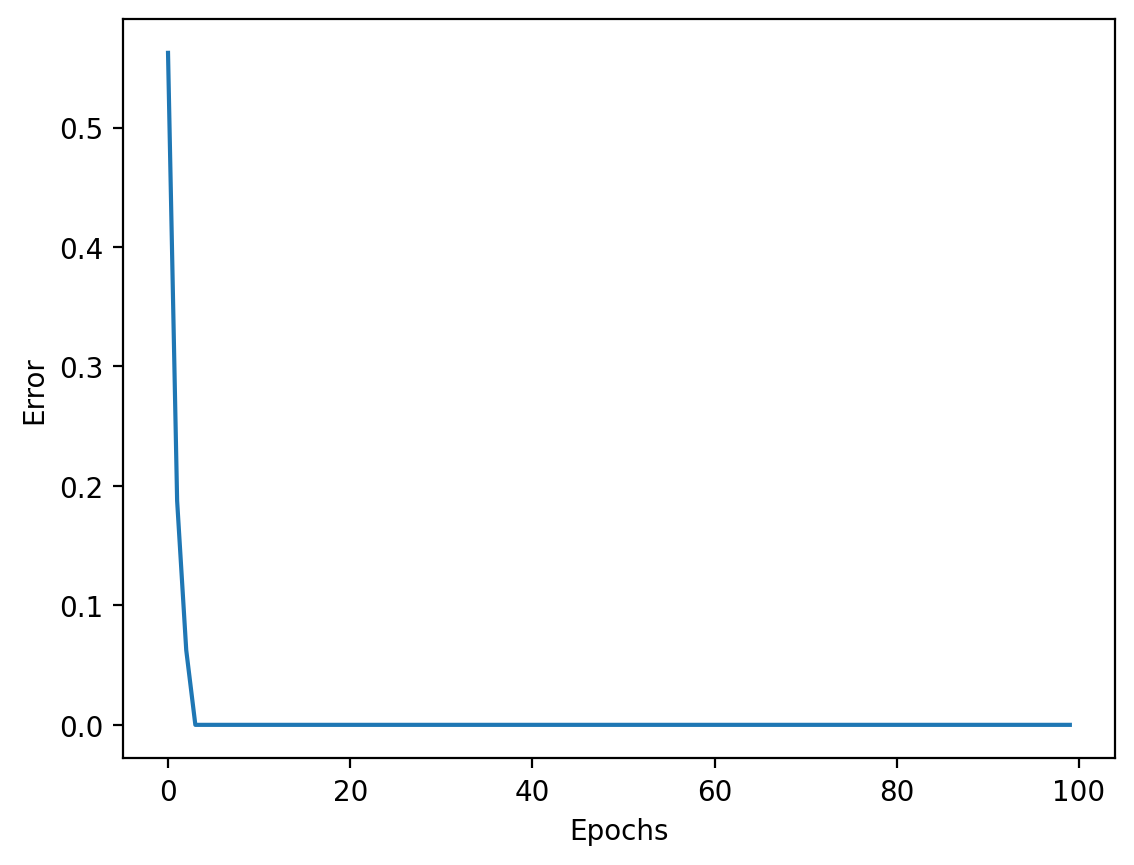
\includegraphics[width=\linewidth]{img/6-training_error.png}
  }
  \caption*{Evolución del error}
  \centering
\end{figure}

\subsection{Capacidad del perceptrón}
El perceptrón simple es capaz de aprender funciones linealmente separables. Una función es linealmente separable si existe un hiperplano que separa los puntos de una clase de los de otra. Tanto la funciones AND y OR de dos entradas como las de cuatro entradas son linealmente separables. A continuación se evalúa la capacidad del perceptrón para estas cuatro funciones, en función de los patrones enseñados. Para eso se calcula el promedio de la tasa de aciertos todos los patrones, de un perceptrón que sólo ve una fracción de los mismos, en cien experimentos. Los resultados se muestran a continuación.
\begin{figure}[H]
  \subcaptionbox*{AND de dos entradas}[.45\linewidth]{
    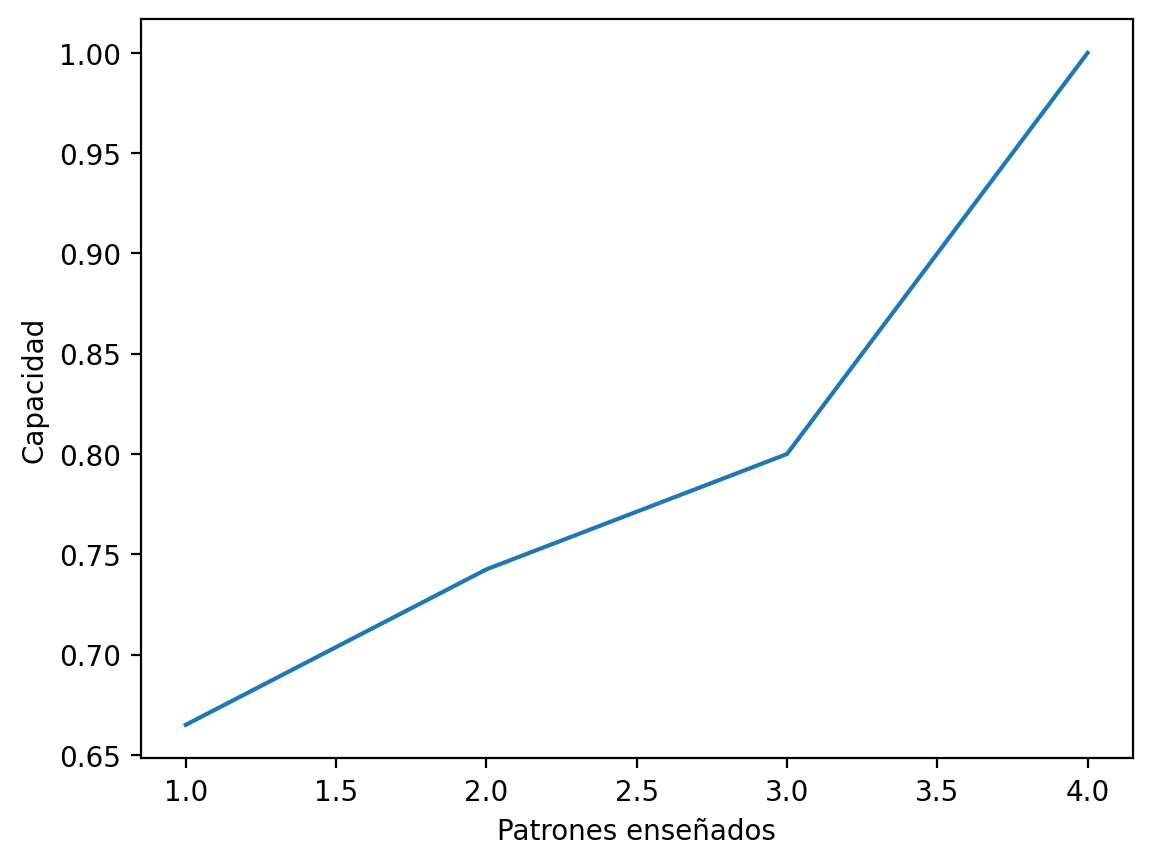
\includegraphics[width=\linewidth]{img/7-capacity.png}
  }
%   \hfill
  \subcaptionbox*{OR de dos entradas}[.45\linewidth]{
    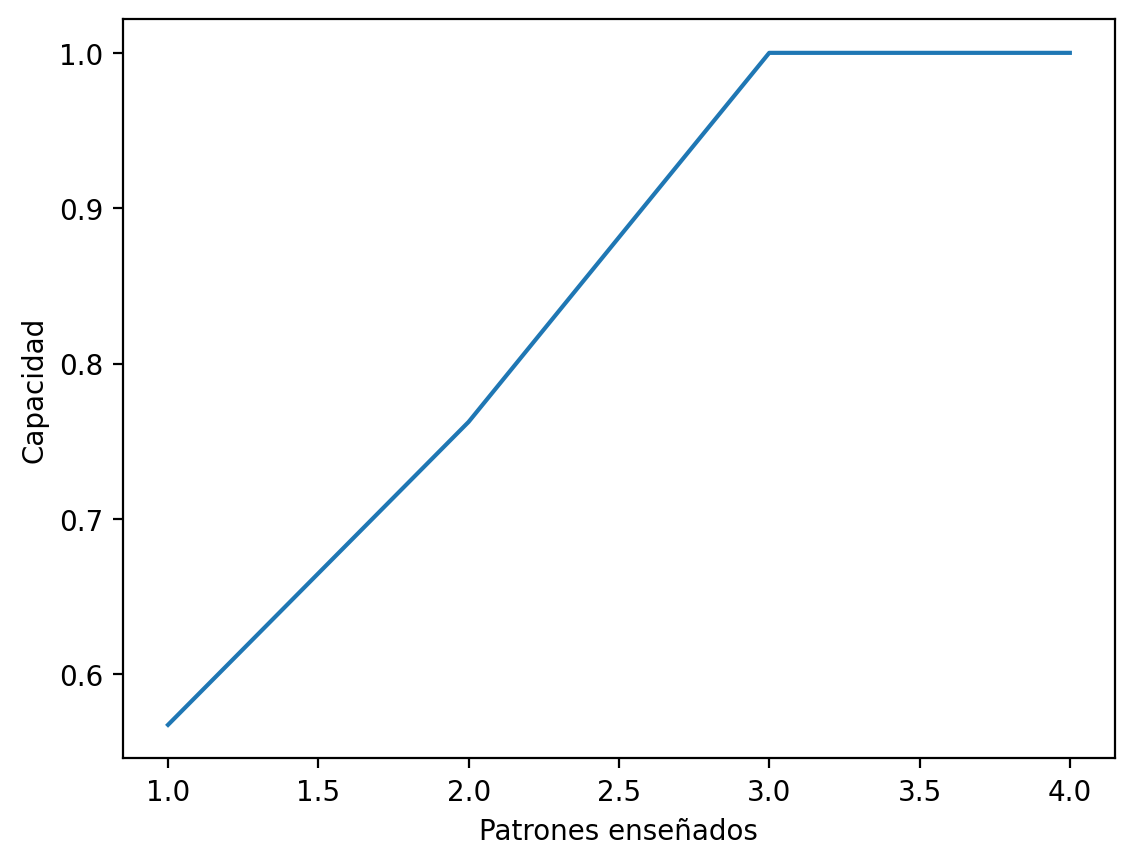
\includegraphics[width=\linewidth]{img/8-capacity.png}
  }
  \caption*{Capacidad}
  \centering
\end{figure}
\begin{figure}[H]
  \subcaptionbox*{AND de cuatro entradas}[.45\linewidth]{
    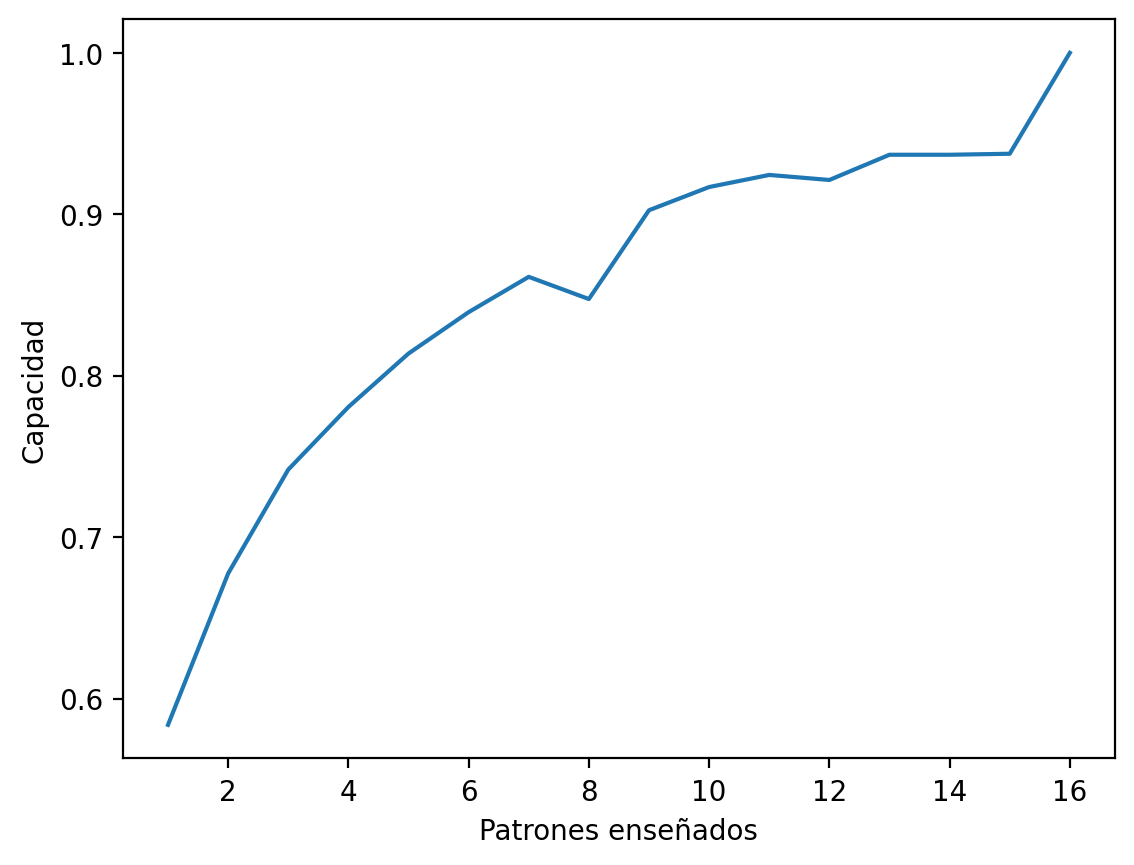
\includegraphics[width=\linewidth]{img/9-capacity.png}
  }
%   \hfill
  \subcaptionbox*{OR de cuatro entradas}[.45\linewidth]{
    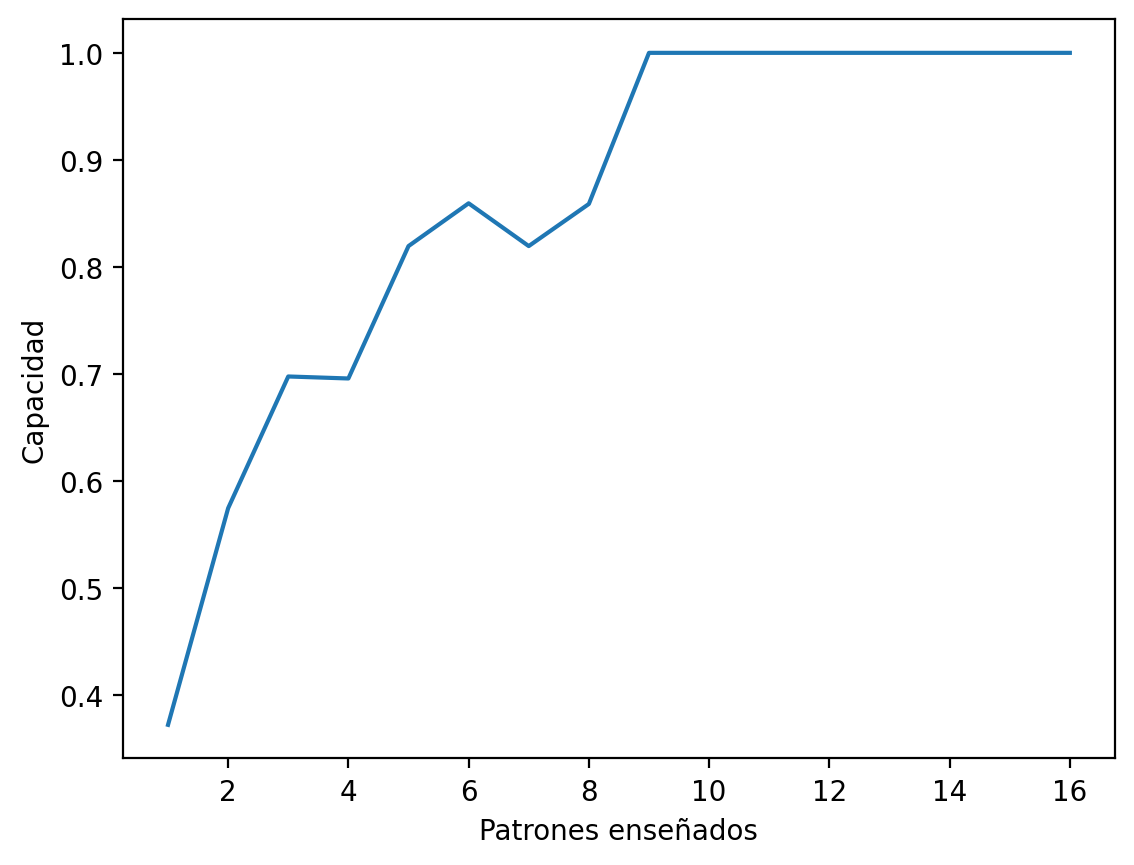
\includegraphics[width=\linewidth]{img/10-capacity.png}
  }
  \caption*{Capacidad}
  \centering
\end{figure}

\newpage
\section{Perceptrón multicapa}
El perceptrón multicapa (MLP) es una red neuronal artificial que consiste en múltiples capas de perceptrones. La idea de un perceptrón multicapa es aproximar una función $f^*$. Por ejemplo, para un clasificador, $y=f^*(\boldsymbol{x})$ mapea una entrada $\boldsymbol{x}$ a una categoría $y$. Un MLP define un mapeo $y=f^*(\boldsymbol{x}, \boldsymbol{\theta})$ y aprende los valores de los parámetros $\boldsymbol{\theta}$ que resultan en la mejor aproximación.
Los MLPs son llamados redes porque generalmente están representados por la composición de distintas funciones. El modelo está asociado con un grafo acíclico que describe cómo las funciones están compuestas.
\begin{figure}[H]
    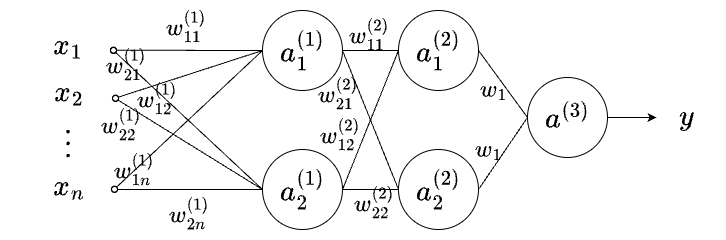
\includegraphics[width=0.7\textwidth]{img/multilayer_perceptron.png}
    \centering
\end{figure}
La salida de un MLP, la activación de su última capa, está dada por la aplicación de la función de activación $\sigma$ a la suma pesada de las activaciones de la capa anterior $a^{(L)}_i = \sigma(\sum_{i=1}^m w^{(L)}_{ij} a^{(L-1)}_j + b^{(L)}_i)$, donde $m$ es la cantidad de nueronas en la capa $L-1$. En forma vectorial:
$$
\begin{aligned}
\boldsymbol{a}^{(L)} &= \sigma(\mathbf{W}^{(L)}\boldsymbol{a}^{(L-1)} + \boldsymbol{b}^{(L)})\\
\boldsymbol{a}^{(L-1)} &= \sigma(\mathbf{W}^{(L-1)}\boldsymbol{a}^{(L-2)} + \boldsymbol{b}^{(L-1)})\\
&\vdots\\
\boldsymbol{a}^{(2)} &= \sigma(\mathbf{W}^{(2)}\boldsymbol{a}^{(1)} + \boldsymbol{b}^{(2)})\\
\boldsymbol{a}^{(1)} &= \sigma(\mathbf{W}^{(1)}\boldsymbol{x} + \boldsymbol{b}^{(1)}),
\end{aligned}
$$
donde $\sigma$ es la función de activación, $\mathbf{W}^{(l)}$ es el conjunto de matrices de pesos de la capa $l$, $\boldsymbol{b}^{(l)}$ es el vector de sesgos de la capa $l$ y $a^{(l)}$ es la activación de la capa $l$, compuesta por las $n$ unidades $a^{(l)}_{1}, a^{(l)}_{2}, \dots, a^{(l)}_{n}$.\\
Para entrenar perceptrón multicapa, se usa el algoritmo del gradiente descendiente. Se calcula el gradiente de la función de pérdida $L = L(y, f(\boldsymbol{x}))$ con respecto a los pesos y sesgos de la red, y se actualizan los parámetros en la dirección opuesta al gradiente, que apunta en la dirección de máximo crecimiento de ésta función. Para calcular el gradiente, se usa el algoritmo de backpropagation, que calcula los gradientes de la función de pérdida con respecto a los pesos y sesgos de la red, propagando el error hacia atrás en la red.\\

\subsection{Backpropagation}
Es útil para definir el algoritmo definir una cantidad intermedia, $\delta^l_j$, que mide el error en el nodo $j$ de la capa $l$.
$$
d^l_j = \frac{\partial L}{\partial z^l_j}.
$$
Las cuatro ecuaciones fundamentales del algoritmo son: el error en la capa de salida $\delta^L$
$$
\delta^L_j = \frac{\partial L}{\partial a^L_j} \sigma'(z^L_j),
$$
que en forma matricial es
\[
\delta^L = \nabla_a L \odot \sigma'(z^L), \label{eq:BP1}\tag{BP1}
\]
donde $\nabla_a L$ es el vector cuyas componentes son las derivadas parciales $\partial L / \partial a^L_j$.
El error $\delta^l$ en función de $\delta^{l+1}$:
\[
\delta^l = ((w^{l+1})^\top \delta^{l+1}) \odot \sigma'(z^l). \label{eq:BP2}\tag{BP2}
\]
Combinando (\ref{eq:BP1}) y (\ref{eq:BP2}) se obtiene $\delta^l$ para cualquier capa en la red.
Una ecuación para la tasa de cambio del costo $L$ con respecto a cualquier sesgo en la red:
\[
\frac{\partial L}{\partial b^l_j} = \delta^l_j. \label{eq:BP3}\tag{BP3}
\]
Por último, una ecuación para la tasa de cambio del costo $L$ con respecto a cualquier peso en la red:
\[
\frac{\partial L}{\partial w^l_{jk}} = a^{l-1}_k \delta^l_j. \label{eq:BP4}\tag{BP4}
\]
El algoritmo backpropagation queda entonces definido de la siguiente manera:
\begin{algorithm}
    1. {\bf Entrada $x$:} Inicializar las activaciones $a^{(1)}$ para la capa de entrada.\\
    2. {\bf Feedforward:} Para cada capa $l=2,3,\dots,L$ calcular $z^{(l)} = w^{(l)} a^{(l-1)} + b^{(l)}$ y $a^{(l)} = \sigma(z^{(l)})$.\\
    3. {\bf Error en la salida $\delta^{(L)}$:} Computar el vector $\delta^{(L)} = \nabla_a L \odot \sigma'(z^{(L)})$.\\
    4. {\bf Retropropagación del error:} Para cada capa $l=L-1, L-2, \dots, 2$ computar $\delta^{(l)} = ((w^{(l+1)})^\top \delta^{(l+1)}) \odot \sigma'(z^{(l)})$.\\
    5. {\bf Salida:} El gradiente de la función de pérdida con respecto a los pesos y sesgos de la red está dado por $\frac{\partial L}{\partial w^{(l)}_{jk}} = a^{(l-1)}_k \delta^{(l)}_j$ y $\frac{\partial L}{\partial b^{(l)}_j} = \delta^{(l)}_j$.
\end{algorithm}

\subsection{Función XOR}
Se entrenaron perceptrones multicapa para que aprendieran las funciones lógicas XOR de dos y cuatro entradas. Para esto se utilizó el algoritmo de gradient descent actualizando en mini batches, junto con backpropagation para calcular los gradientes correspondientes. Se usaron dos capas ocultas, con 3 neuronas cada una, la función de activación $\tanh$, y dos capas ocultas, de 5 neuronas cada una, con la función de activación $\tanh$, respectivamente. Los resultados se muestran a continuación:
\begin{figure}[H]
  \subcaptionbox*{XOR de dos entradas}[.45\linewidth]{
    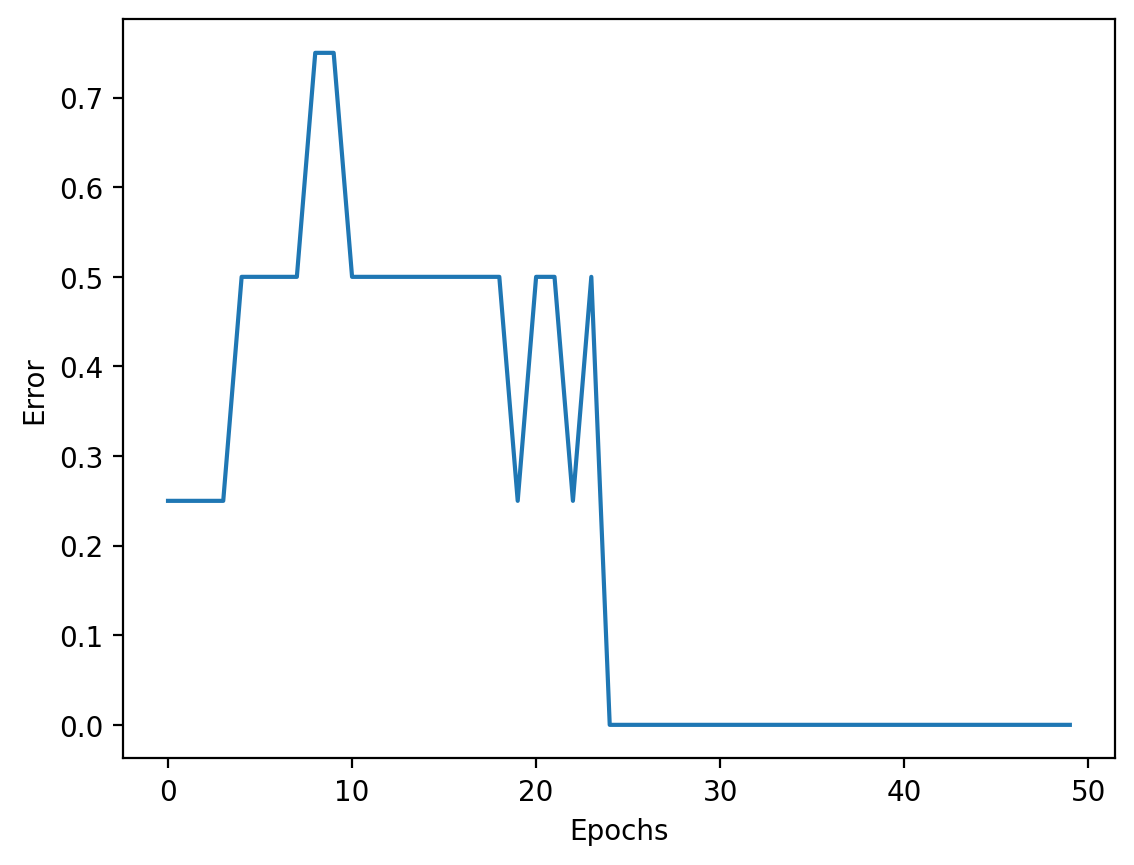
\includegraphics[width=\linewidth]{img/11-training_error.png}
  }
%   \hfill
  \subcaptionbox*{XOR de cuatro entradas}[.45\linewidth]{
    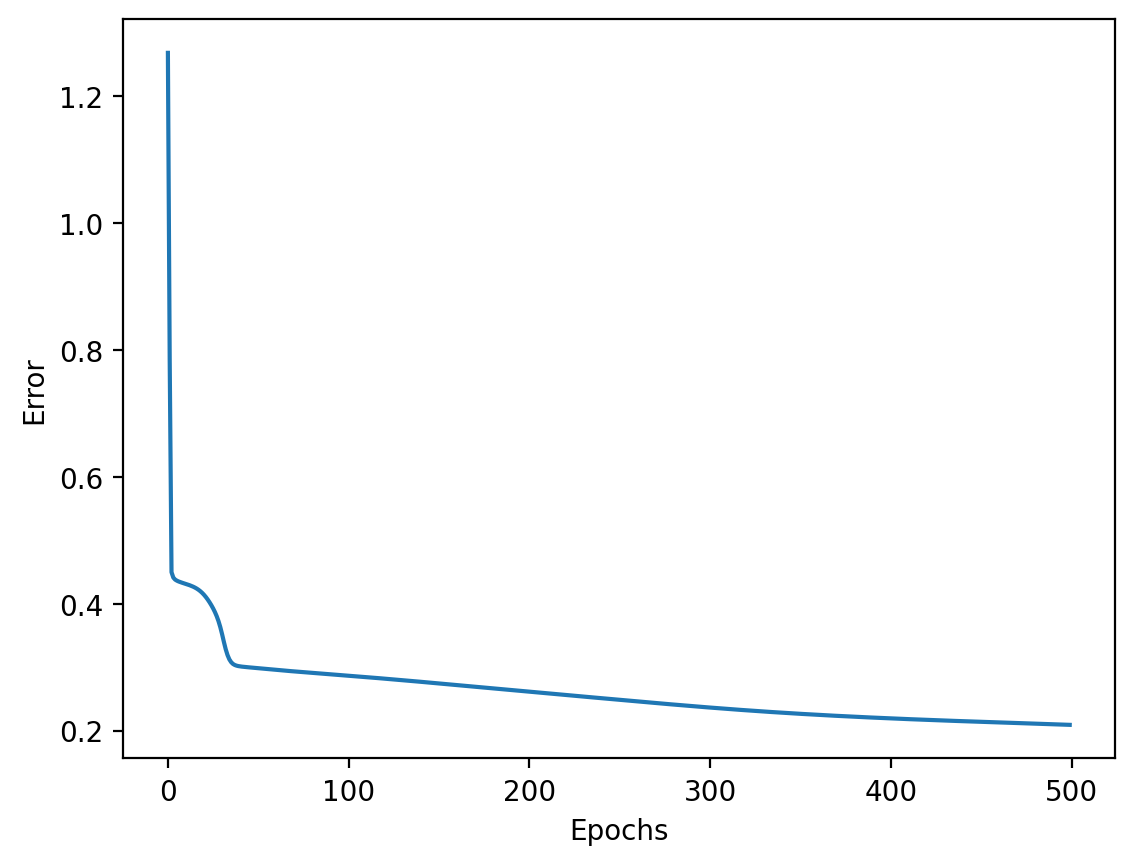
\includegraphics[width=\linewidth]{img/12-training_error.png}
  }
  \caption*{Evolución del error}
  \centering
\end{figure}

\subsection{Suma de lineal y trigonométricas}
A continuación, se muestran los resultados obtenidos de la evaluación del perceptrón ante la función $f(x,y,z) = \sin x + \cos y + z$, con $x$ e $y \in [0,2\pi]$ y $z \in [-1,1]$. Para esto se construyó un set de datos de entrenamiento y otro para evaluación, y se analizó la evolución del error en ambos sets a lo largo del entrenamiento. Primero se usaron dos capas ocultas con nueve neuronas cada una:
\begin{figure}[H]
    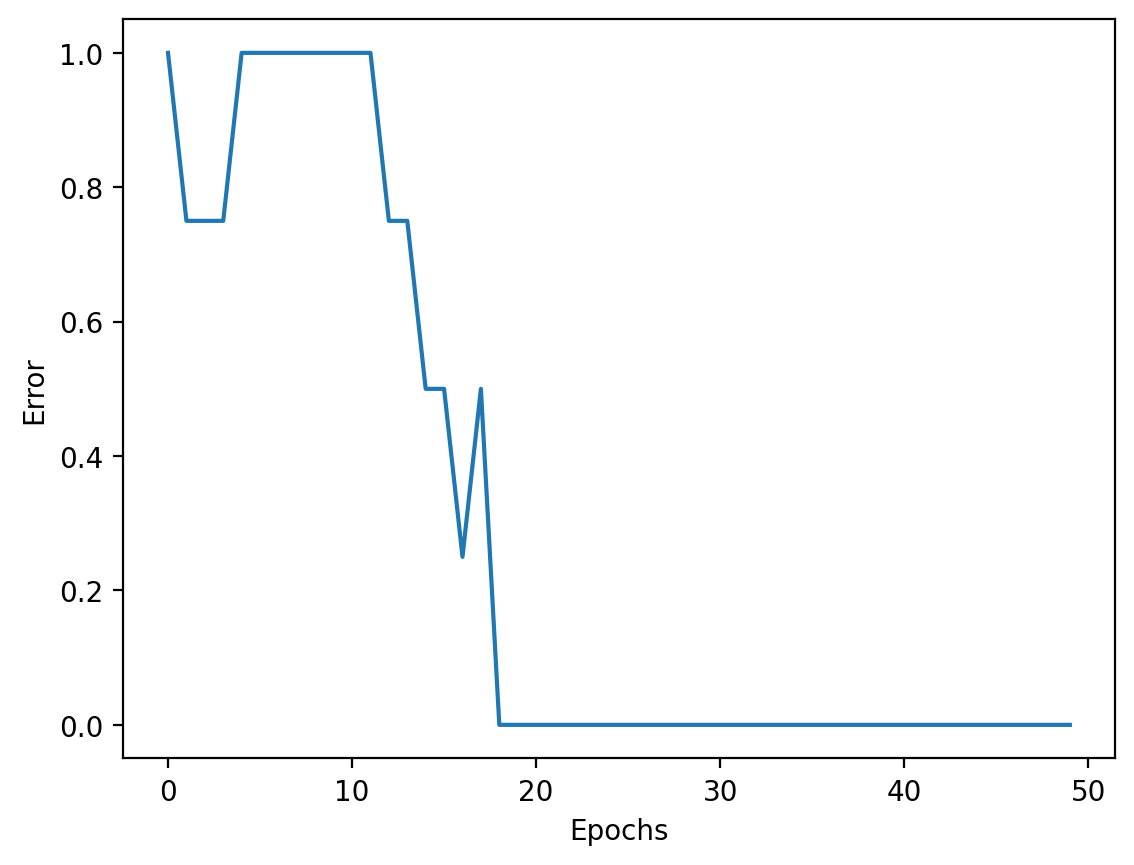
\includegraphics[width=0.7\textwidth]{img/13-training_error.png}
    \centering
\end{figure}
Luego se analizó el mismo problema para una red con una única capa oculta con un conjunto de entrenamiento de 40 muestras, para mini batches de 40 y 1 muestra.
\begin{figure}[H]
    \subcaptionbox*{Mini batch de 40 muestras}[.45\linewidth]{
        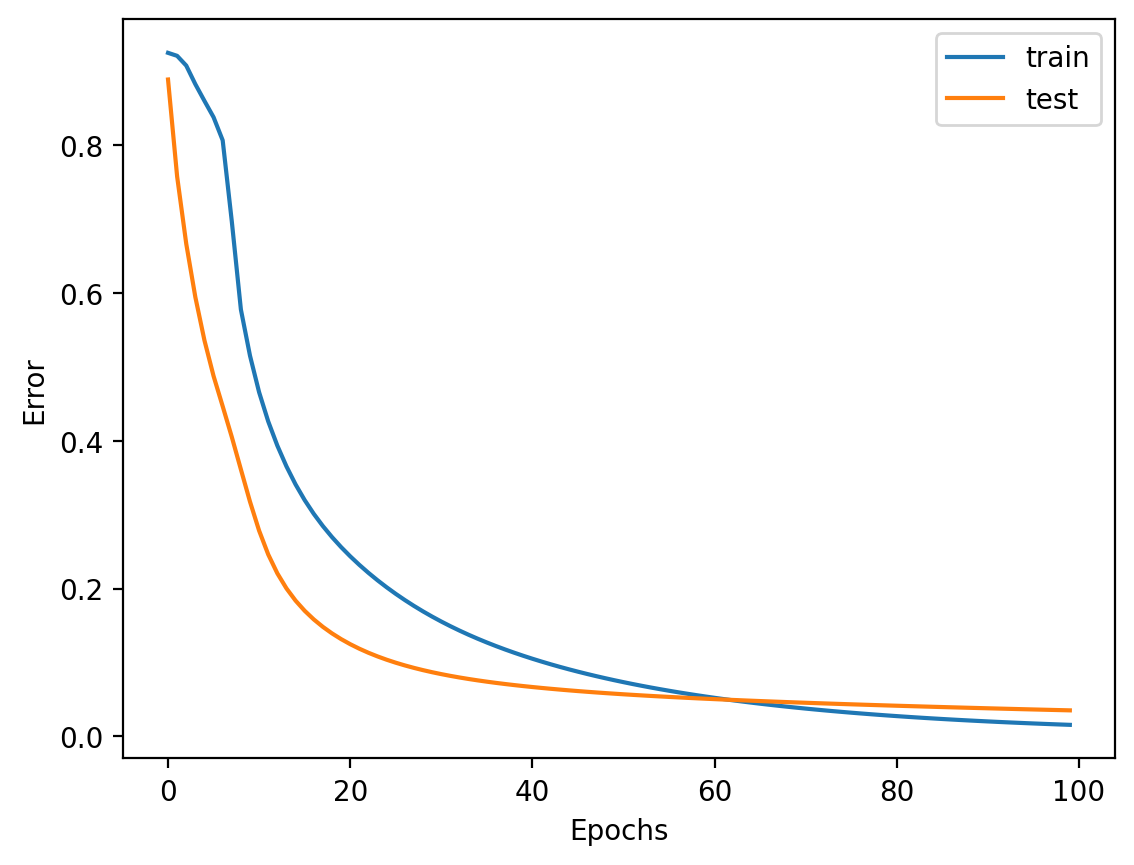
\includegraphics[width=\linewidth]{img/14-training_error.png}
    }
    \subcaptionbox*{Mini batch de 1 muestra}[.45\linewidth]{
        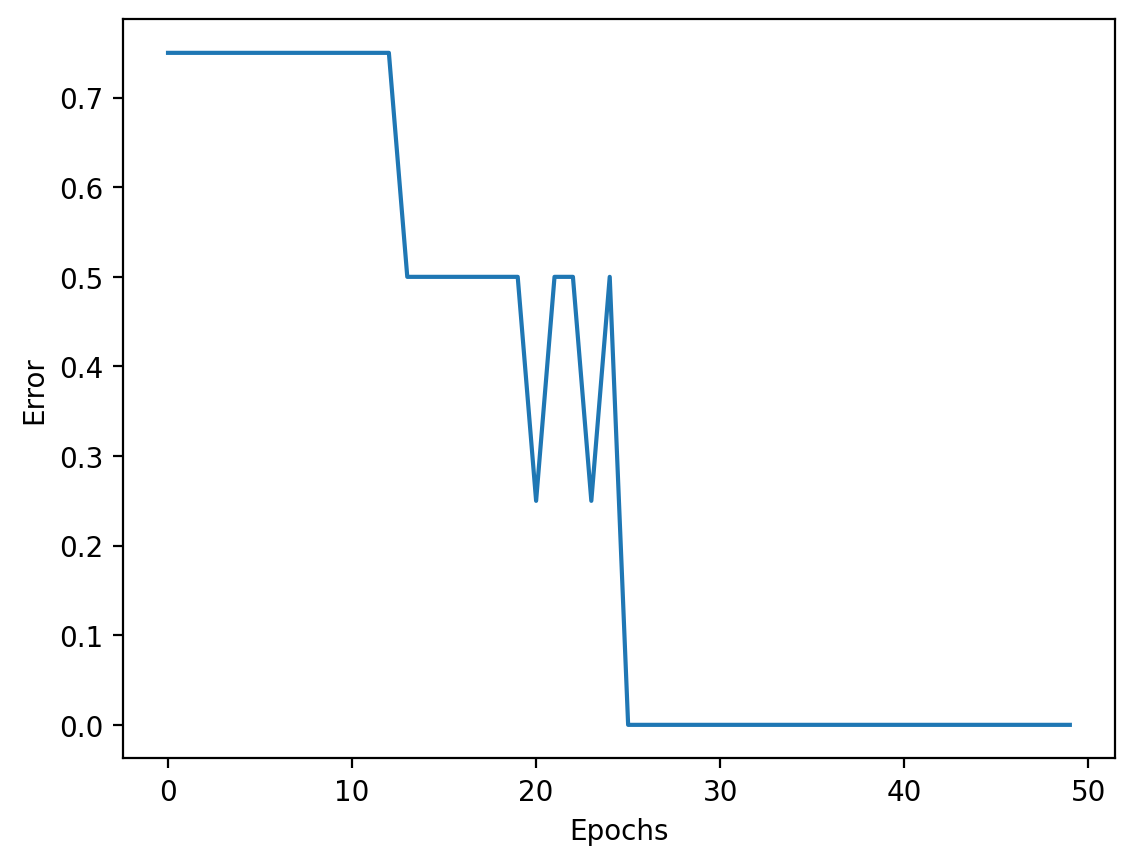
\includegraphics[width=\linewidth]{img/15-training_error.png}
    }
\end{figure}
% quizás debería hacer algún análisis de éste último resultado

\newpage
\section{Máquina restringuida de Boltzmann}
% Una máquina de Boltzmann es un modelo basado en energía, definimos la probabilidad conjunta usando una función de energía (distribución de Boltzmann)
% $$
% P(\boldsymbol{x}) = \frac{\exp(-E(\boldsymbol{x}))}{Z},
% $$
% donde $E(\boldsymbol{x}) es la función de energía y $Z$ es la función de partición que asegura que $\sum_\boldsymbol{x} P(\boldsymbol{x}) = 1$.\\
% La función de energía de la máquina de Boltzmann es
% $$
% E(\boldsymbol{x}) = -\boldsymbol{x}^\top \boldsymbol{U} \boldsymbol{x} - \boldsymbol{b}^\top \boldsymbol{x},
% $$
% donde $\boldsymbol{U}$ es la matriz de pesos y $\boldsymbol{b}$ es el vector de sesgos.\\
Las máquinas restringuidas de Boltzmann (RBMs) son uno de los pilares fundamentales de los modelos estocásticos profundos. Las RBMs son modelos estocásticos profundos indireccionales que contienen una capa de variables observables y una capa de variables latentes. Las RBMs pueden ser apiladas para generar modelos más profundos.\\
Una máquina de Boltzmann es un grafo bipartito completo, las unidades del modelo pueden ser divididas en dos grupos, en los que las unidades no están interconectadas, pero sí lo están con todas las unidades del otro grupo.\\
La RBM se un modelo basado en energía, con la probabilidad conjunta definida por su función de energía (distribución de Boltzmann):
$$
P(\mathbf{v} = \boldsymbol{v}, \mathbf{v} = \boldsymbol{h}) = \frac{\exp(-E(\boldsymbol{v}, \boldsymbol{h}))}{Z},
$$
donde $E$ es la funciónd de energía, definida
$$
E(\boldsymbol{v}, \boldsymbol{h}) = -\boldsymbol{b}^\top \boldsymbol{v} - \boldsymbol{c}^\top \boldsymbol{h} - \boldsymbol{v}^\top \boldsymbol{W} \boldsymbol{h},
$$
y $Z$ es la constante de normalización conocida como función de partición
$$
Z = \sum_{\boldsymbol{v}} \sum_{\boldsymbol{h}} \exp(-E(\boldsymbol{v}, \boldsymbol{h})).
$$
De la definición, es aparente que calcular la constante de normalización $Z$ (sumar exhaustivamente todos los estados) es computacionalmente intractable. Para el caso de las máquinas de Boltzmann, esta afirmación está demostrada formalmente. Pero existe la posibilidad de calcularla más rápido aprovechando regularidades en la función de probabilidad, las probabilidades condicionales $P(\mathbf{h}|\mathbf{v})$ y $P(\mathbf{v}|\mathbf{h})$ son factoriales y relativamente simples de computar y de muestrear. Más aún, las distribuciones factoriales dadas la capa oculta y la capa visible son
$$
\begin{aligned}
P(\boldsymbol{h}|\boldsymbol{v}) &= \prod_{j=1}^{n_h} \sigma\left((2\boldsymbol{h} - 1) \odot (\boldsymbol{c} + \boldsymbol{W}^\top \boldsymbol{v})\right)_j,\\
P(\boldsymbol{v}|\boldsymbol{h}) &= \prod_{j=1}^{n_v} \sigma\left((2\boldsymbol{v} - 1) \odot (\boldsymbol{b} + \boldsymbol{W} \boldsymbol{h})\right)_i.
\end{aligned}
$$

\subsection{Preentrenamiento}
En el trabajo de Hinton y Salakhutdinov (2006) se propuso un algoritmo de preentrenamiento para RBMs. El agoritmo surge de que gradient descent puede ser utilizado para hacer un reajuste fino de los pesos siempre y cuando los pesos se encuentren inicialmente en un estado cercano a una solución.\\
La idea es hacer que el modelo aprenda una representación de baja dimensionalidad de los datos, usando un \textbf{encoder} multicapa que transofmra los datos de alta dimensionalidad en un código de baja dimensionalidad y en \textbf{decoder} similar que reconstruye los datos originales a partir del código.\\
Si partimos de pesos aleatorios en ambas redes, pueden ser entrenadas en conjunto mediante la minimización de la discrepancia entre la entrada y la reconstrucción, usando por ejemplo gradient descent con backpropagation. El sistema en conjunto tiene el nombre de \textbf{autoencoder}.
Es difícil optimizar los pesos en un autoencoders no lineales que tienen múltiples capas ocultas. Con pesos iniciales altos, generalmente malos mínimos locales son encontrados; con pesos iniciales bajos, los gradientes son demasiado pequeños para entrenar autoencoders profundos. Por otro lado, si los pesos están cerca de una buena solución, el gradiente descendiente funciona bien.
El algoritmo de preentrenamiento consiste en varias partes. Primero, la probabilidad de de una imagen del set de entrenamiento puede ser aumentada ajustando los pesos y sesgos para disminuir la energía de la esa imagen y aumentar la energía de las imágenes similares "confabuladas" que la red prefiere en vez de los datos reales. Dada una imagen de entrenamiento, el estado binario $h_j$ de cada detector de features $j$ se pone en $1$ con probabilidad $\sigma(b_j+\sum_i v_i w_{ij})$, donde $\sigma$ es la función sigmoide $1/(1+\exp(-x))$, $b_j$ es el sesgo de $j$, $v_i$ es el estado del pixel $i$ y $w_{ij}$ es el peso entre $i$ y $j$.
Una vez elegidos los estados binarios de las unidades ocultas, se produce una confabulación activando (poniendo en $1$) cada $v_i$ con probabilidad $\sigma(b_i + \sum_j h_j w_{ij})$, donde $b_i$ es el sesgo de $i$. Luego se actualizan una vez más los estados de las capas ocultas para que representen features de la confabulación. El cambio en cada peso está dado por
$$
\Delta w_{ij} = \epsilon(\langle v_i h_j \rangle_\text{data} - \langle v_i h_j \rangle_\text{recon}),
$$
donde $\epsilon$ es la taza de aprendizaje, $\langle v_i h_j \rangle_\text{data}$ es la fracción de veces que el pixel $i$ y la el detector de features $j$ están activados en simultáneo cuando los detectores de features están siendo estimulados por los datos de entrenamiento, y $\langle v_i h_j \rangle_\text{recon}$ es la correspondiente fracción de tiempo para las confabulaciones.\\
Luego de aprender una capa de detectores de features, podemos tratar sus actividades cuando están siendo estimulados por los datos de entrenamiento como datos de entrada para aprender una segunda capa de features. Luego la primer capa de detectores de features se convierte en la capa visible para la próxima RBM.\\
Este entrenamiento capa por capa puede repetirse arbitrariamente. Se puede mostrar que añadir una capa extra siempre mejora la cota inferior de la log-verosimilitud de que el modelo asigna a los datos de entrenamiento, siempre que el número de detectores de features por capa no disminuzca y siempre que sus pesos se inicialicen correctamente.\\
Cada capa de features captura fuertes correlaciones entre las actividades de las unidades en la capa anterior.
Luego de preentrenar múltiples capas de detectores de features, el modelo se despliega para producir un encoder y un decoder que incialmente usan los mismos pesos. La etapa de reajuste fino global reemplaza entonces las actividades estocásticas por probabilidades reales determinísticas y usa backpropagation sobre todo el autoencoder para realizar el ajsute fino de los pesos para lograr una reconstrucción óptima.
Para datos continuos, las unidades ocultas de la RBM de la primera capa siguen siendo binarias, pero las unidades visibles son reemplazadas por unidades lineales con ruido gaussiano. Si el ruido tiene varianza unitaria, la regla estocástica de actualización para las unidades ocultas permanece entonces igual y la regla de actualización para cada unidad visible $i$ es simplemente muestrear de una gaussiana con varianza unitaria y media $b_i + \sum_j h_j w_{ij}$.\\
\subsection{Reconstrucción de MNIST}
Se entrenó una pila de RBMs para reconstruir imágenes del set de datos MNIST. Se usaron tres máquinas restruinguidas de Boltzmann con 600, 400 y 200 unidades ocultas por capa respectivamente, con 784 unidades visibles en la primer máquina, siendo que las imágenes del set son de 72 por 72 pixeles. El algoritmo utilizado para el aprendizaje es el de preentrenamiento descripto en el paper de Hinton y Salakhutdinov. A continuación se muestra la evolución de los errores de entrenamiento en mil épocas, usando como métrica de error la suma de los errores absolutos en cada pixel, y la reconstrucción de imágenes del set para cada clase del mismo junto a las imágenes originales.
\begin{figure}[H]
    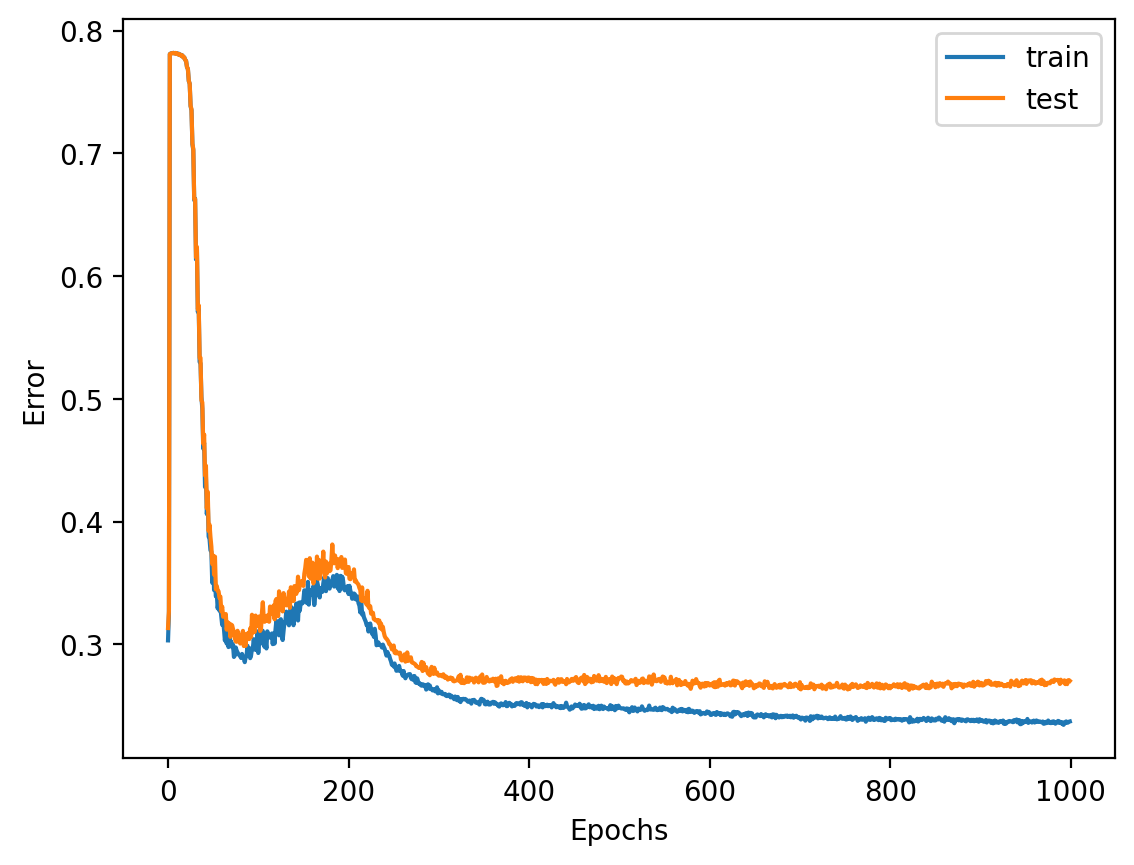
\includegraphics[width=0.7\textwidth]{img/16-training_error.png}
    \centering
    \caption*{Evolución del error}
\end{figure}
\begin{figure}[H]
    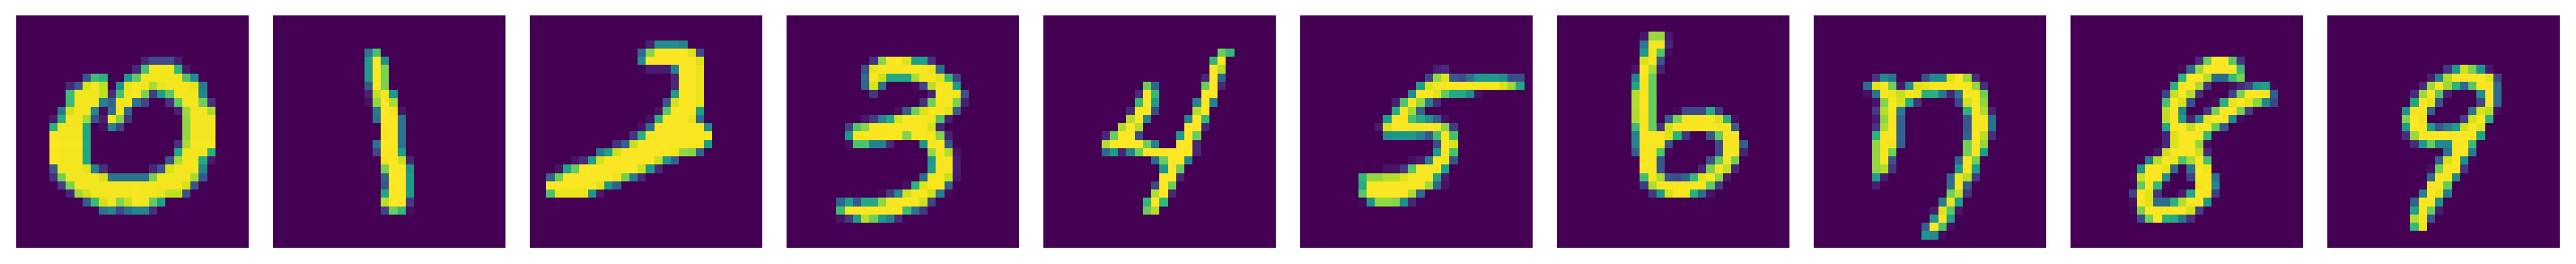
\includegraphics[width=\linewidth]{img/17-original_images.png}
    \centering
    \caption*{Imágenes originales}
\end{figure}
\begin{figure}[H]
    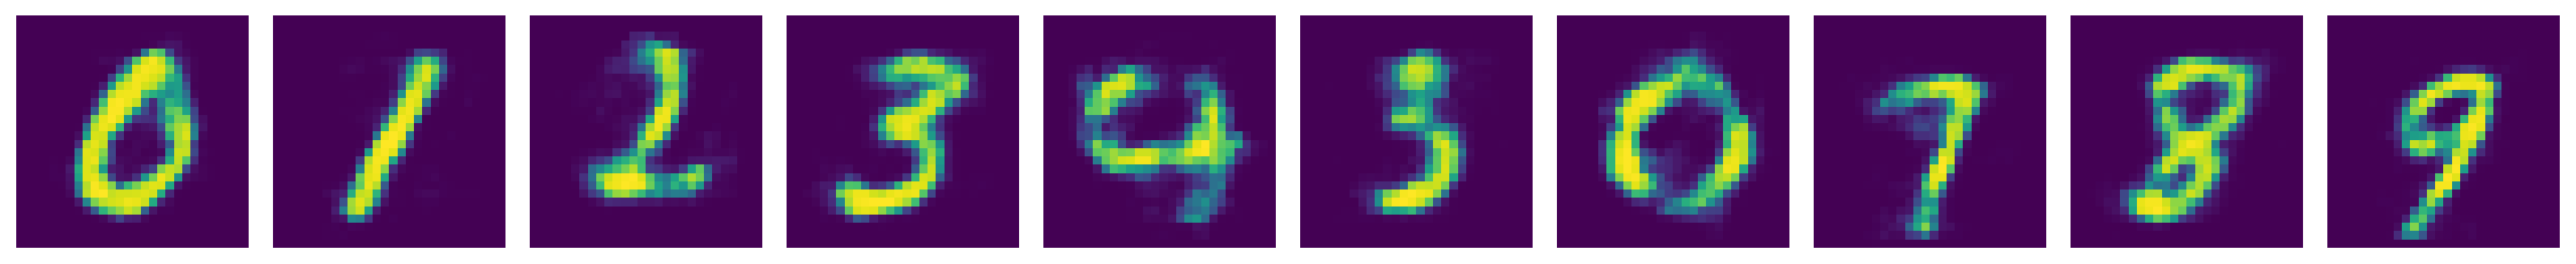
\includegraphics[width=\linewidth]{img/18-reconstructions.png}
    \centering
    \caption*{Reconstrucciones}
\end{figure}

\section{Red convolucional}
Las redes convolucionales o redes neuronales convolucionales (CNNs), son una especie especial de redes neuronales para procesar datos que tienen una topología de cuadrícula conocida.
El nombre red convolucional indica que la red emplea una operación matemática llamada convolución, que es una especie particular de operación lineal.
En una CNN, la entrada es un tensor de dimensión
$$
\text{cantidad de entradas} \times \text{altura de la entrada} \times \text{ancho de la entrada} \times \text{cantidad de canales},
$$
luego de pasar por una capa convolucional, la imagen se abstrae a un mapa de features, con dimensiones
$$
\text{cantidad de entradas} \times \text{altura del mapa} \times \text{ancho del mapa} \times \text{cantidad de canales del mapa}.
$$

% Bibliografía
\newpage
\begin{thebibliography}{9}
% \bibitem{ejemplo} Autor, \emph{Título del libro}, Editorial, Año.
\bibitem{Deep Learning} Ian Goodfellow. Yoshua Bengio. Aaron Courville, \emph{Deep Learning}.
\bibitem{Neural Networks and Deep Learning} Michael Nielsen, \emph{Neural Networks and Deep Learning}.
\bibitem{Reducing the Dimensionality of Data with Neural Networks} G. E. Hinton. R. R. Salakhutdinov, \emph{Reducing the Dimensionality of Data with Neural Networks}.
\bibitem{Object Recognition with Gradient-Based Learning} Yann LeCun. Patrick Haffner. Léon Bottou. Yoshua Bengio, \emph{Object Recognition with Gradient-Based Learning}.

\end{thebibliography}

\end{document}

